\documentclass[twocolumn]{aastex62}
\usepackage{graphicx}
\usepackage{subfigure}
\usepackage{multirow}
\newcommand{\vdag}{(v)^\dagger}
\newcommand\aastex{AAS\TeX}
\newcommand\latex{La\TeX}

%% Reintroduced the \received and \accepted commands from AASTeX v5.2
%% Command to document which AAS Journal the manuscript was submitted to.
%% Adds "Submitted to " the arguement.
\submitjournal{ApJ}

\def\ie{{\it i.e. }}
\def\eg{{\it e.g. }}
\def\etc{{\it etc}}

\shorttitle{Include the Extreme Faint Galaxy in Shear Measurement}
\shortauthors{Hekun Li et al.}


\begin{document}

\title{Including the Extremely Faint Sources in the Shear Measurement}


\correspondingauthor{Jun Zhang}
\email{betajzhang@sjtu.edu.cn}

\author{Hekun Li}
\affiliation{Department of Physics and Astronomy, Shanghai Jiao Tong University, Shanghai 200240, China}
\author{Jun Zhang*}
\affiliation{Department of Physics and Astronomy, Shanghai Jiao Tong University, Shanghai 200240, China}


\begin{abstract}



\end{abstract}


\keywords{gravitational lensing: weak-methods: data analysis, extremely low SNR}


\section{Introduction} \label{sec:intro}

The large structure in the dark matter field perturbs the light passing through and introduces a slight but coherent distortion to the observed shapes of background galaxies. This effect is called weak gravitational lensing or cosmic shear. The statistical analysis of weak gravitational lensing is one of the most promising probes for the large structure mass distribution, the expansion history of the universe, \etc\citep{Bartelmann2001, Hoekastra2008,Kilbringer2015}. The ongoing large weak lensing surveys, such as DES \citep{Troxel2018}, KIDS \citep{Hildebrandt2016}, and HSC \citep{Hikage2019}, and the next generation surveys, such as LSST \citep{Abell2009} and Euclid \citep{Laureijs2011}, will accumulate a great amount of galaxy images for the improvement of shear measurement accuracy from one percent to sub-percent level, and, therefore, constrain the cosmological parameters more stringently. 

The shear measurement is currently subject to many systematic errors, such as modeling bias \citep{Bernstein2010,Voigt2010,Kacprzak2014}, noise bias \citep{Refregier2012,Kacprzak2014}, and selection bias \citep{Hirata2003}, which should be controlled carefully to achieve the sub-percent level precision. 

noise bias, 

precision achieved

cite the previous paper, cut and calibration to avoid bias

cut -- suppress noise bias -- selection bias


We focus on the Fourier\_Quad method\citep{Zhang2008, Zhang2015} in this paper to investigate the effect of noise on measurement precision. The Fourier\_Quad method is a moment-based method that measures the shape from the Fourier transform of the galaxy image without any assumption of the galaxy morphology. \cite{Zhang2017} propose a non-weighted statistical approach for shear recovery, the PDF\_SYM approach, which utilizes the full PDF of the non-weighted shear estimators from both faint and bright galaxies to achieve a lower statistical error bound. Recently, we find the PDF\_SYM approach would be slightly biased by the extremely faint sources. The typical magnitude of the multiplicative (additive) bias would reach $\sim 10^{-2}$ ($10^{-4}$) level at SNR $\sim 10$. However, the bias vanishes on the high SNR end. In this paper, we aim to find the origin of the bias and appropriate correction to it. In Section \ref{sec:FQ}, we briefly introduce the Fourier\_Quad method and the statistical approaches for shear recovery. We investigate the bias origin in the Section \ref{sec:bias_cal}, and present the correction in Section \ref{sec:bias_corr}.

%\cite{Zhang2015} have shown that the statistical approach for shear recovery of Fourier\_Quad is non-biased even at SNR $\sim5$. However, when applied to a real shear measurement, it needs appropriate weights to suppress the scatter from the magnitude difference between the faint and bright galaxies. A non-biased weight is generally difficult to obtain from the noisy image.


 



\section{The Fourier\_Quad method}\label{sec:FQ}
%introduce the details of shear measurement, average approach
The Fourier\_Quad is a model-independent shear measurement method that estimates the shape of a galaxy based on its 2D power spectrum \citep{Zhang2008, Zhang2015, Zhang2017}. The shear estimators are defined as:
\begin{eqnarray}
\label{shear_estimator}
G_1&=&-\int d^2\vec{k}(k_x^2-k_y^2)T(\vec{k})M(\vec{k})\\ \nonumber
G_2&=&-2\int d^2\vec{k}k_xk_yT(\vec{k})M(\vec{k})\\ \nonumber
N&=&2\int d^2\vec{k}\left[k^2-\frac{\beta^2}{2}k^4\right]T(\vec{k})M(\vec{k}), \\ \nonumber
U &=& -\beta^2\int d^2\vec{k}(k_x^4 - 6k_x^2k_y^2 + k_y^4)T(\vec{k})M(\vec{k}), \\ \nonumber
V &=& -4\beta^2\int d^2\vec{k}(k_x^3k_y - k_xk_y^3)T(\vec{k})M(\vec{k}).
\end{eqnarray}
The $M(\vec{k})$ is the power spectrum of the galaxy image from which the background and Poisson noise have been subtracted through:
\begin{eqnarray}
\label{FQ_TM}
&&M(\vec{k})=\left\vert\widetilde{f}_I(\vec{k})\right\vert^2-F_I-\left\vert\widetilde{f}_B(\vec{k})\right\vert^2+F_B\\ \nonumber
&&F_I=\frac{\int_{\vert\vec{k}\vert > k_c} d^2\vec{k}\left\vert\widetilde{f}_I(\vec{k})\right\vert^2}{\int_{\vert\vec{k}\vert > k_c} d^2\vec{k}}, \;\;\; F_B=\frac{\int_{\vert\vec{k}\vert > k_c} d^2\vec{k}\left\vert\widetilde{f}_B(\vec{k})\right\vert^2}{\int_{\vert\vec{k}\vert > k_c} d^2\vec{k}},
\end{eqnarray}
where $\widetilde{f}_I(\vec{k})$ and $\widetilde{f}_B(\vec{k})$ are the Fourier transformations of the galaxy image and a neighboring image of background noise respectively. $F_B$ and $F_I$ are the estimates of the Poisson noise power spectrum of the background noise and source images respectively. A critical wavelength, $k_c$, is required to avoid the contamination of the source power\citep{Zhang2015}. The factor $T(\vec{k})$ is the ratio of power spectrum of the target isotropic Gaussian PSF (point spread function) to that of the original PSF, $T(\vec{k}) = |\widetilde{W}_{\beta}(\vec{k})|^2/|\widetilde{W}_{P}(\vec{k})|^2$.
It is designed to coverts the original PSF, $W_{P}(\vec{x})$, to an isotropic Gaussian PSF, $W_{\beta}(\vec{x})$, so that the effect of PSF can be corrected rigorously and model-independently.
%\begin{equation}
%W_{\beta}(\vec{x})=\frac{1}{2\pi \beta^2}\exp\left[-\frac{|\vec{x}|^2}{2\beta^2}\right]
%\end{equation}
The scale radius, $\beta$, of $W_{\beta}(\vec{x})$ should be chosen slightly larger than that of $W_{P}(\vec{x})$ to avoid the singularities in the factor $T(\vec{k})$. 

Fourier\_Quad method provides two statistical approaches for shear recovery from the estimators, the average approach, and the PDF\_SYM approach. The former approach recovers the shear signal by taking ensemble averages of the shear estimators:
\begin{eqnarray}
\label{mean}
\frac{1}{2}\frac{\left\langle  G_1\right\rangle }{\left\langle  N\right\rangle }=g_1+O(g_{1,2}^3),\;\;\;\frac{\left\langle  G_2\right\rangle }{\left\langle  N\right\rangle }=g_2+O(g_{1,2}^3).
\end{eqnarray}
It is precise to the second order of shear in accuracy\citep{Zhang2015}. \cite{Zhang2015} have shown the appealing advantage of Fourier\_Quad that including the extreme faint sources or even point sources would not bias the shear measurement. An appropriate weight should be considered in Eq.\ref{mean} because the bright galaxies will dominate in the ensemble average and enlarge the estimate of the error bar. However, a non-biased weight is generally difficult to obtain from the noisy image.

To approach the lower statistical error bound, \cite{Zhang2017} propose a non-weighted shear recovery method in the Fourier\_Quad framework which is called the PDF\_SYM approach. It recovers the shear signal by symmetrizing the probability distribution function (PDF) of the shear estimators. \cite{Zhang2017} show that the PDF of $\hat{G}_{1/2}$ would be maximally symmetrical respect to zero if the shear estimate, $\hat{g}_{1/2}$ is the true one (see \cite{Zhang2017} for more details). 
\begin{eqnarray}
\hat{G}_{1} = G_1 - \hat{g}_{1}(N + U), \;
\hat{G}_{2} = G_2 - \hat{g}_{2}(N - U).
\end{eqnarray}
It needs two additional shear estimators, $U$ and $V$. The $V$ term is kept for the rotation with $U$. The PDF\_SYM approach estimates each component of shear ($g_1$ or $g_2$) independently. Therefore, when estimating one component, it is convenient to ignore the other one or set it zero.   

Unlike the weighted sum of shear estimators used by the other methods, the PDF\_SYM approach includes the full PDF of the shear estimators and does not weight down the faint sources. Therefore, it could make full use of the additional information from faint sources to achieve a lower statistical error. The PDF\_SYM approach would be a promising method for shear recovery in the Fourier\_Quad framework.

Recently, we find the PDF\_SYM approach would be biased by the extremely faint galaxies. Figure \ref{fig:pts_mc} shows the multiplicative and additive bias measured from the samples of different SNR levels. The multiplicative bias could reach about $1\%$ level when the SNR is about $10$. We find the PSF anisotropy ($e \sim 0.1$) would induce additive bias ($\sim 6\times 10^{-4}$) to the measurement at the same SNR level. The bias would vanish on the high SNR end. However, the average approach is immune to this bias even applied to the extremely noisy sample. The results above are measured from the galaxy sample of different SNR generated by the random walk method. The merit of the random walk method includes precise shape distortion, less computational cost, and efficient PSF convolution (see \cite{Li2020} for more details of the random walk method and image simulation setup).


\begin{figure*}[htbp]
	\centering
	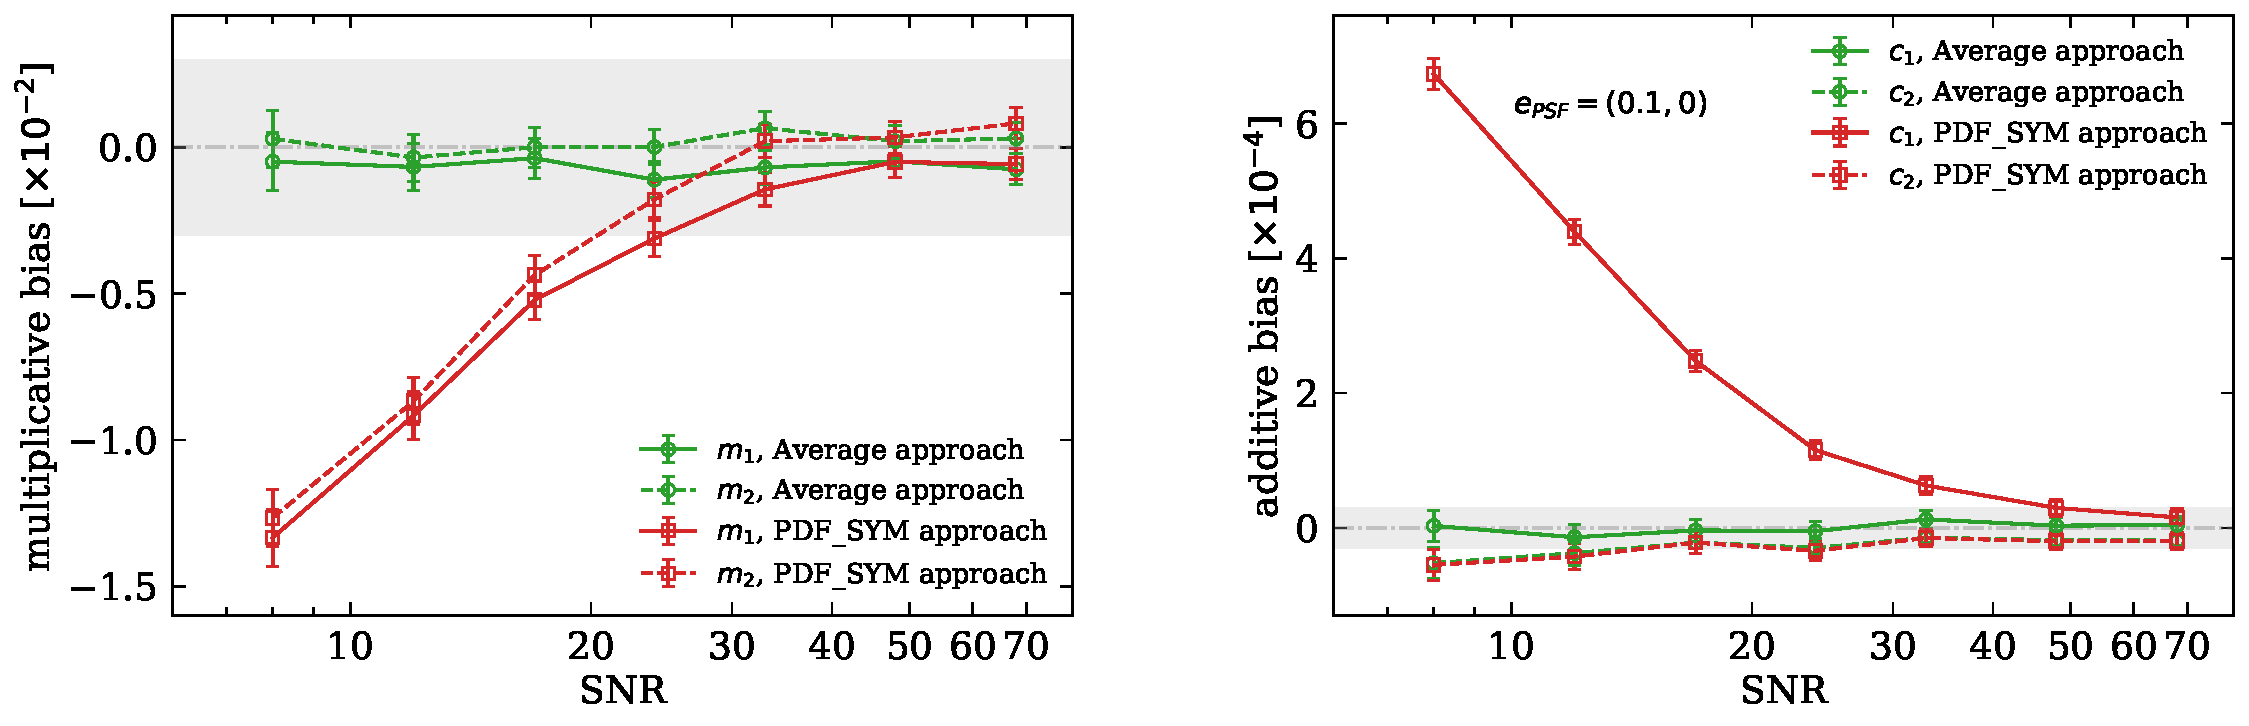
\includegraphics[width=0.9\linewidth]{figures/pts_sample_mc.pdf}
	\caption{The multiplicative and additive bias measured from the galaxy of different SNR level. The shaded region in the left (right) panel is between $\pm 3\times 10^{-3}$ ($\pm 3\times10^{-5}$). }\label{fig:pts_mc}
\end{figure*}


\section{Bias caused by the source and noise mix}\label{sec:bias_cal}
To reveal the underlying origin of the bias, we should start from the components of noisy galaxy image which could be written as a sum of source and noise image, \ie$f_I(\vec{x}) = f_G(\vec{x}) + f_N(\vec{x})$. The modified power spectrum of the noisy galaxy image, $M(\vec{k})$, can be rewritten as 
\begin{eqnarray}
M(\vec{k}) =  \left\vert\widetilde{f}_G(\vec{k})\right\vert^2+ C(\vec{k}) + \Delta N(\vec{k}).
\end{eqnarray}
The first term is the power spectrum of the noise-free source image. $C(\vec{k})$ is the mixture term of the Fourier transform of the source and that of the background noise. $\Delta N(\vec{k})$ is the noise power spectrum residual after the background noise subtraction. 
\begin{eqnarray}
& C(\vec{k})& = \widetilde{f}_{G}^{*}(\vec{k})\widetilde{f}_N(\vec{k}) + \widetilde{f}_{G}(\vec{k})\widetilde{f}_{N}^{*}(\vec{k}),\\ \nonumber
&\Delta N(\vec{k})& = \left\vert\widetilde{f}_N(\vec{k})\right\vert^2 -\left\vert\widetilde{f}_B(\vec{k})\right\vert^2.
\end{eqnarray}
We have dropped the estimate of the Poisson noise power spectrum, $F_S$ and $F_B$, because they are not important here. 

In the image simulation, we test different combinations of the components from $M(\vec{k})$. We find that the noise power spectrum residual, $\Delta N(\vec{k})$, would not bias the measurement. While, the result will be biased if the $C(\vec{k})$ term is included in the measurement. Furthermore, we find that both multiplicative and additive bias will vanish when $\vert \widetilde{W}_{P}(\vec{k})\vert$ rather than $\vert \widetilde{W}_{P}(\vec{k})\vert^2$ is used in the PSF deconvolution ($T(\vec{k})$ factor) for the $C(\vec{k})$. We present the comparison in Figure \ref{fig:pts_componets}.

\begin{figure*}[htbp]
	\centering
	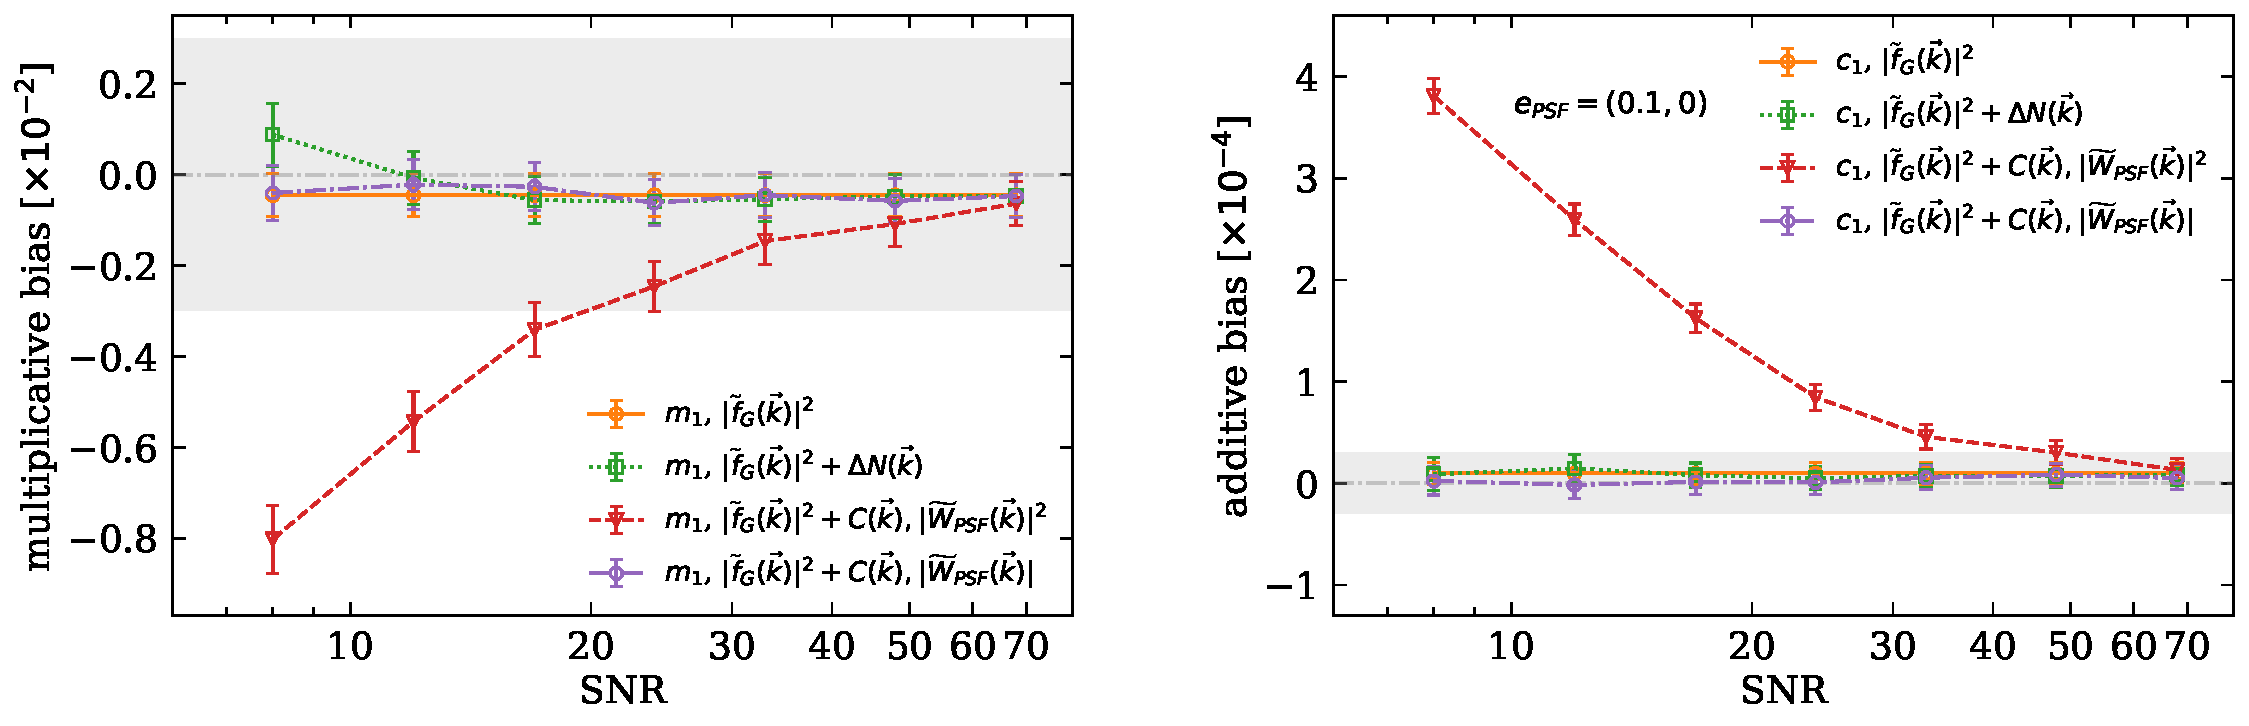
\includegraphics[width=0.9\linewidth]{figures/pts_sample_components.pdf}
	\caption{The multiplicative and additive bias at different SNR levels measured by the original PDF\_SYM from different components of the power spectrum of the noisy galaxy image. To avoid the overlap between curves, only the $m_1$'s and $c_1$'s curves are shown. Orange curves: Measured from the power spectrum of the noise-free galaxy image. Green curves: Measured from the combination of noise-free part and the noise power spectrum residual, $\Delta N(\vec{k})$. Red curves: Measured from the combination of noise-free galaxy image power spectrum and the Fourier transform mixture, $C(\vec{k})$. The PSF power spectrum, $\vert \widetilde{W}_{P}(\vec{k})\vert^2$, is used for deconvolution. Purple curves: Same components are used for measurement as the red curves. However, $\vert \widetilde{W}_{P}(\vec{k})\vert$ is used (in $T(\vec{k})$) in PSF deconvolution for $C(\vec{k})$.}\label{fig:pts_componets}
\end{figure*}

To understand the bias mechanism, we should consider the contribution of $C(\vec{k})$ to the shear estimators in Eq.(\ref{shear_estimator}). For the simplicity in calculation, let $f_k$ and $n_k$ denotes the Fourier transform of noise free source image and that of the background noise image respectively. Assuming that the PDF\_SYM approach has been applied, we obtain
\begin{eqnarray}
\label{Eq:gg}
\hat{G}_1&=&\int{d}^2\vec{k} P_k T(\vec{k})\left(\vert f_k\vert^2 + C(\vec{k})\right) \\ \nonumber
&=&\Delta^2\sum_k A_k \left(\vert f_k\vert^2+2f_k^{Re}n_k^{Re}+2f_k^{Im}n_k^{Im}\right), \\ \nonumber
\hat{G}_2&=&\int{d}^2\vec{k} \; Q_k T(\vec{k})\left(\vert f_k\vert^2 + C(\vec{k})\right)\\ \nonumber
&=&\Delta^2\sum_kB_k\left(\vert f_k\vert^2+2f_k^{Re}n_k^{Re}+2f_k^{Im}n_k^{Im}\right),
\end{eqnarray}
where
\begin{eqnarray}
&&A_k = P_k T(\vec{k}),\; B_k = Q_k T(\vec{k}) ,\\ \nonumber
P_k = k_x^2-k_y^2&& + \hat{g}_1\left[2k^2-\beta^2\left(k^4+k_x^4-6k_x^2k_y^2+k_y^4\right)\right],\\ \nonumber
Q_k = 2k_xk_y+&&\hat{g}_2\left[2k^2-\beta^2\left(k^4-k_x^4+6k_x^2k_y^2-k_y^4\right)\right].
\end{eqnarray}
Here, we have dropped the notation of integral variation for simplicity and rewritten the integration into the discrete form. $\Delta^2$ is the integral surface element.

For a certain galaxy, let us consider the PDF of $\hat{G}_1$ and $\hat{G}_2$ with many the background noise realizations. Assuming that the noise is mainly white noise, the PDF of $n_k^{Re}$ and $n_k^{Im}$ should be a normal distribution which is independent of $\vec{k}$. The standard deviation is assume to be $\sigma$. Then, the PDF of $\hat{G}_1$ and $\hat{G}_2$ is given by\footnote{The details of calculation in this section can be found in Appendix \ref{app}.}:
\begin{eqnarray}
\label{Eq:Pgg_1}
P_G\left(\hat{G}_1,\hat{G}_2\right)=\frac{1}{(2\pi)^2}\frac{\pi}{\sqrt{D}}\exp\left[-\frac{C}{4D}\right]
\end{eqnarray}
where
\begin{eqnarray}
\label{Eq:Pgg_2}
C &=& \left(\hat{G}_1-\Gamma_1\right)^2U_3+\left(\hat{G}_2-\Gamma_2\right)^2U_1 \\ \nonumber
&&-2\left(\hat{G}_1-\Gamma_1\right)\left(\hat{G}_2-\Gamma_2\right)U_2,\\ \nonumber
D&=& U_1U_3-U_2^2,\\ \nonumber
\left(\Gamma_1,\Gamma_2\right)&=&\Delta^2\sum_k\vert f_k\vert^2\left(A_k,B_k\right)\\ \nonumber
\left(U_1,U_2,U_3\right)&=&2\sigma^2\Delta^4\sum_k\vert f_k\vert^2\left(A_k^2,A_kB_k,B_k^2\right)
\end{eqnarray}

The $1$-D PDF of $\hat{G}_1$($\hat{G}_2$) is needed by the PDF\_SYM approach for $g_1$($g_2$) estimating. Therefore, for example, let us consider the PDF of $\hat{G}_1$. By integrating the $\hat{G}_2$, we would have
\begin{eqnarray}
\label{1d_PDF}
&&\int_{-\infty}^{\infty}d\hat{G}_2 P_G\left(\hat{G}_1,\hat{G}_2\right)\\ \nonumber
&=&\frac{1}{(2\pi)^2}\frac{\pi\sqrt{\pi}}{\sqrt{U_1}}\exp\left\{-\frac{\left(\hat{G}_1-\Gamma_1\right)^2}{4U_1}\right\}
\end{eqnarray}
where
\begin{eqnarray}
\Gamma_1&=&\int{d}^2\vec{k}\;\left(k_x^2-k_y^2\right)\exp(-\beta^2k^2)\vert f_S(\vec{k})\vert^2, \\ \nonumber
U_1&=&2\sigma^2\Delta^2\int{d}^2\vec{k} \; \left(k_x^2-k_y^2\right)^2\exp(-2\beta^2k^2)\frac{\vert f_S(\vec{k})\vert^2}{\vert \widetilde{W}_{P}(\mathrm{M}\vec{k})\vert^2}, \\ \nonumber
\mathrm{M}&=&\left[\begin{array}{cc}
1-g_1 &  -g_2 \\
-g_2 &  1+g_1 
\end{array}\right]
\end{eqnarray}
We have assumed that the $1$-D PDF of $\hat{G}_1$ has been symmetrized by the true shear signal. Therefore, any asymmetry part, which should vanish, in the PDF will cause the bias. Assuming the ellipticity of the PSF is ($e_1$,$e_2$), and suppose the components are small. For convenience in the rest of our discussion, we set $g_2=0$, and the ellipticity $e_2$ of the PSF is also zero. Then, we can expand the power spectrum of PSF to the first order of $g_1$ and $e_1$.
\begin{eqnarray}
\vert \widetilde{W}_{P}(\mathrm{M}&&\vec{k})\vert^{-2} \\ \nonumber
&&= W^{-2}W^\prime [2(e_1+g_1)(k_x^2-k_y^2)]
+W^{-1}.
\end{eqnarray}
$W$ is the abbreviation of $\vert \widetilde{W}_{P}(\vec{k})\vert^{-2}$, and $W^\prime$ is first order derivative to $W$.
Therefore, we can rewrite the functions of $\Gamma_1$ and $U_1$ as:
\begin{eqnarray}
U_1&=&U_{10}+\delta U,\\ \nonumber
\Gamma_1&=&\int kdk\int d\theta \exp(-\beta^2k^2)\vert f_S(k,\theta)\vert^2k^2\cos(2\theta),
\end{eqnarray}
where
\begin{eqnarray}
U_1 &=& 2\sigma^2\Delta^2\int kdk\int d\theta\exp(-2\beta^2k^2) \\ \nonumber
&&\times\vert f_S(k,\theta)\vert^2W^{-1}k^4 \cos^2(2\theta), \\ \nonumber
\delta U &=& 2\sigma^2\Delta^2\int kdk\int d\theta\exp(-2\beta^2k^2) \\ \nonumber
&&\times\vert f_S(k,\theta)\vert^2\left[ 2(e_1+g_1)W^{-2}W^\prime k^6\cos^3(2\theta)\right].
\end{eqnarray}
Considering to the first order of $\delta U$, we could write the $1$-D PDF of $\hat{G}_1$ as:
\begin{eqnarray}
\label{1d_PDF}
&&\int_{-\infty}^{\infty}d\hat{G}_2 P_G\left(\hat{G}_1,\hat{G}_2\right)\\ \nonumber
&\approx&\frac{1}{(2\pi)^2}\frac{\pi\sqrt{\pi}}{\sqrt{U_{10}}}\left[1-\frac{\delta U}{2U_{10}}+\frac{\left(\hat{G}_1-\Gamma_1\right)^2}{4U_{10}}\frac{\delta U}{U_{10}}\right] \\ \nonumber &\times&\exp\left\{-\frac{\left(\hat{G}_1-\Gamma_1\right)^2}{4U_{10}}\right\}
\end{eqnarray}
The terms proportional to $\delta U$, when averaged over galaxies, generate the asymmetry of $P_G$. 

It should be noted that $U_1$ is derived from the $C(\vec{k})$ which only contains $\widetilde{f}_G(\vec{k})$ not the power spectrum $\vert\widetilde{f}_G(\vec{k})\vert^2$. Therefore, the PSF deconvolution (the factor $T(\vec{k}) = |\widetilde{W}_{\beta}(\vec{k})|^2/|\widetilde{W}_{P}(\vec{k})|^2$) will give rise to an additional factor, $1/\vert W_{P}(\mathrm{M}\vec{k})\vert^2$, in $U_1$. However, the PSF is appropriately removed from the $\Gamma_1$ which is derived from the power spectrum of source image. So the appropriate PSF deconvolution for $C(\vec{k})$, the mixture of Fourier transform of the galaxy image and background image, is the origin of bias. See Appendix \ref{app} for more details.



%Figure \ref{fig:pts_componets} shows that the mixture of galaxy image Fourier transform and that of the background noise image, $\left\vert C(\vec{k})\right\vert^2$, causes both multiplicative and additive bias in the measurement. Furthermore, only the PDF\_SYM approach is biased by $\left\vert C(\vec{k})\right\vert^2$.





\section{Improvement to the sub-percent precision}\label{sec:bias_corr}
Although an appropriate PSF deconvolution for the $C(\vec{k})$ term would correct the bias, image components separation could not be achieved in the real data. It should be noted that what we have for measurement are the noisy images and the shear estimators measured from that. Among the components of $M(\vec{k})$, the $C(\vec{k})$ part is the one that easy to estimate. We propose a new method that utilizes the shear estimators from the estimated $C(\vec{k})$ to correct the bias. 

Recall that the original measurement, Eq.(\ref{FQ_TM}), employs the power spectrum of a noise image to subtract the contamination to shear estimators from the background noise. However, this operation leaves an annoying term, $C(\vec{k})$, to the shear measurement. In our new method, we need a second noise image, $f_{B^{\prime}}(\vec{x})$, to estimate this component. Then, we would get the shear estimators from this component by applying the shear measurement to it. There are four steps:
\begin{itemize}
	
	\item Apply the measurement defined in Section \ref{sec:FQ} to get the shear estimators, $G_1$, $G_2$, $N$, $U$, and $V$. This step needs the first noise image.

	\item Add the second noise image to the original noisy galaxy image, $f_S(\vec{x})$, to get a new image, $f_{I^{\prime}}(\vec{x})$.
	\begin{eqnarray}
	f_{I^{\prime}}(\vec{x}) = f_G(\vec{x}) + f_N(\vec{x}) + f_{B^{\prime}}(\vec{x}).
	\end{eqnarray}
	Subtract the power spectrum of the new noise image and that of the original noisy galaxy image from the power spectrum of the new image above.
	\begin{eqnarray}
	C^{\prime}(\vec{k})=&&\left\vert \widetilde{f}_{I^{\prime}}(\vec{x})\right\vert^2 - \left\vert \widetilde{f}_{I}(\vec{x})\right\vert^2 - \left\vert \widetilde{f}_{B^{\prime}}(\vec{x})\right\vert^2 \\ \nonumber
	 =&& \widetilde{f}_{G}^{*}(\vec{k})\widetilde{f}_{B^{\prime}}(\vec{k}) + \widetilde{f}_{G}(\vec{k})\widetilde{f}_{B^{\prime}}^{*}(\vec{k}).
	\end{eqnarray}
	The noise-noise power mixture, $\widetilde{f}_{N}^{*}(\vec{k})\widetilde{f}_{B^{\prime}}(\vec{k}) + \widetilde{f}_{N}(\vec{k})\widetilde{f}_{B^{\prime}}^{*}(\vec{k})$, has been neglected because we find it would not change the result in our new method.
	
	\item Rotate the PSF image by $90$ degrees in the measurement to cancel out the additive bias induced by the anisotropy of PSF. The image rotation changes the factor $T(\vec{k})\rightarrow T'(\vec{k})=\vert \widetilde{W}_\beta(\vec{k})\vert^2 /\vert \widetilde{W}_P^{\perp}(\vec{k})\vert^2$. $\vert \widetilde{W}_P^{\perp}(\vec{k})\vert^2$ is the power spectrum of rotated PSF image. Apply the shear measurement to $C^{\prime}$ to get the new shear estimator: $\Delta G_1$ and $\Delta G_2$.
	\begin{eqnarray}
	\Delta G_1&=&\int{d}^2\vec{k}\left(k_x^2-k_y^2\right)T'(\vec{k}) C^{\prime}(\vec{k}), \\ \nonumber
	\Delta G_2&=&\int{d}^2\vec{k}\left(2k_xk_y\right)T'(\vec{k}) C^{\prime}(\vec{k}).
	\end{eqnarray}
	\item Rotate ($\Delta G_1$, $\Delta G_2$) by $45$ degrees and add it to the original shear estimator ($G_1$, $G_2$). 
	\begin{equation}
	\left[ \begin{array}{ccc}
	G_1^{new} \\
	G_2^{new} \\
	\end{array} 
	\right ] = 
		\left[ \begin{array}{ccc}
	G_1 \\
	G_2 \\
	\end{array} 
	\right ]
	+
	\left[ \begin{array}{ccc}
		0 & -1 \\
		1 & 0\\
		\end{array} 
	\right ]
	\left[ \begin{array}{ccc}
	\Delta G_1 \\
	\Delta G_2 \\
	\end{array} 
	\right ]
	\end{equation}
\end{itemize}
Then, one would get the unbiased shear signal by applying the PDF\_SYM approach to symmetrize the PDF of $G_{1/2}^{new} - \hat{g}_{1/2}(N+/-)U$. We present the comparison of the original PDF\_SYM approach and the improved one in Figure \ref{fig:pts_mc_corr}. We test the new PDF\_SYM approach against a more realistic image simulation in which the Magnitude of galaxies ranges from $22$ to $25$. Table \ref{tb:real_simu} shows the comparison.

\begin{table}
\centering
\caption{}\label{tb:real_simu}
\begin{tabular}{ccc}
	\multicolumn{3}{c}{Improvement in a realistic image simulation} \\
	\hline 
	\hline 
	& Multiplicative bias& Additive bias \\ 
	& $10^3m_{1/2}$& $10^4c_{1/2}$ \\
	\hline 
	\multirow{2}{*}{Original PDF\_SYM}&  $-6.08(\pm0.67)$&  $3.26(\pm0.16)$\\ 
	&  $-5.95(\pm0.67)$&  $-0.23(\pm0.16)$\\ 
	\hline 
	\multirow{2}{*}{New PDF\_SYM}&  $-0.09(\pm0.74)$&  $-0.11(\pm0.17)$\\ 
	&  $0.77(\pm0.74)$&  $-0.15(\pm0.17)$\\ 
	\hline 
\end{tabular}
\end{table} 

\begin{figure*}[htbp]
	\centering
	\includegraphics[width=0.9\linewidth]{figures/pts_sample_corr.pdf}
	\caption{The multiplicative and additive bias measured by different statistical approaches from the samples of different SNR. For each SNR level, the multiplicative bias is corrected to smaller than $3\times10^{-3}$ by the new PDF\_SYM approach. The residual of additive bias is $\sim 5\times10^{-5}$ for the smaples of SNR lower than $15$.}\label{fig:pts_mc_corr}
\end{figure*}


To understand the how this correction works, let us consider the PDF, $P_{\Delta}(\Delta G_1,\Delta G_2)$. Following the same strategy for $P_G(\hat{G}_1,\hat{G}_2)$, we have\footnote{The details of calculation in this section can be found in Appendix \ref{app}.}
\begin{eqnarray}
&&P_{\Delta}\left(\Delta G_1,\Delta G_2\right)
=\frac{1}{(2\pi)^2}\frac{\pi}{\sqrt{D^\prime}}\exp\left[-\frac{C^\prime}{4D^\prime}\right], \\ \nonumber
&&\quad C^\prime = \Delta G_1^2V_3-2\Delta G_1\Delta G_2V_2+\Delta G_2^2V_1, \\ \nonumber
&&\quad D^\prime = V_1V_3-V_2^2.
\end{eqnarray}
The parameters, $V_1$, $V_2$, and $V_3$ are defined as
\begin{eqnarray}
&&V_1 = 2\sigma^2\Delta^2\int{d}^2\vec{k}\left(k_x^2-k_y^2\right)^2 M^\prime(\vec{k}),\\ \nonumber
&&V_2 = 2\sigma^2\Delta^2\int{d}^2\vec{k}2k_xk_y\left(k_x^2-k_y^2\right)M^\prime(\vec{k}),\\ \nonumber
&&V_3 = 2\sigma^2\Delta^2\int{d}^2\vec{k}(2k_xk_y)^2 M^\prime(\vec{k}),\\ \nonumber
&&M^\prime(\vec{k})=\exp(-2\beta^2k^2)\vert f_S(\mathrm{M}^{-1}\vec{k})\vert^2\frac{\vert W_{P}(\vec{k})\vert^2}{\vert W_{P}^{\perp}(\vec{k})\vert^4}.
\end{eqnarray}
Compared with $\hat{G}_{1/2}$, the $\Delta G_{1/2}$ contains different noise component which could be regarded as a scatter. Therefore, after adding the $\Delta G_{1/2}$ to the original $\hat{G}_{1/2}$, the new PDF of $\hat{G}_1$ and $\hat{G}_2$ could be written as a convolution between the $P_G(\hat{G}_1,\hat{G}_2)$ and $P_{\Delta}(\Delta G_1,\Delta G_2)$. Then, we can write down the corresponding $1$-D PDF, $P_F(\hat{G}_1)$, as
\begin{eqnarray}
P_F&&(\hat{G}_1)\\ \nonumber
&&=\int d\hat{G}_2\int d\Delta G_1\int d\Delta G_2  P_{\Delta}(-\Delta G_2,\Delta G_1)\\ \nonumber 
&&\quad \times P_G(\hat{G}_1-\Delta G_1,\hat{G}_2-\Delta G_2)\\ \nonumber
&&=\frac{8\pi^3\sqrt{\pi}}{(2\pi)^4}\frac{1}{\sqrt{U_1+V_3}}\exp\left\{-\frac{(\hat{G}_1-\Gamma_1)^2}{4(U_1+V_3)}\right\},
\end{eqnarray}
where
\begin{eqnarray}
U_1&& + V_3\\ \nonumber
=&&2\sigma^2\Delta^2\int kdk\int d\theta\exp(-2\beta^2k^2)\vert f_S(k,\theta)\vert^2\\ \nonumber
&&\times W^{-1}\left\{{g_1k^6[(\beta^2+2W^{-1}W')\cos(2\theta)-\beta^2\cos(6\theta)]}\right.\\ \nonumber
&&\left.{+2e_1k^6\cos(6\theta)W^{-1}W'+k^4}\right\} \\ \nonumber
=&&\delta_{N_s}+N_s
\end{eqnarray}
$N_s$ is a scalar, and $\delta_{N_s}$ is a perturbation made of quantities of spin-2 and spin-6. In the 1-D PDF given by $P_F(\hat{G}_1)$, $\Gamma_1$ can be treated as a small quantity comparing to $\hat{G}_1$, as the bias is important only for galaxies of very small signal-to-noise ratios\footnote{According to Eq.(\ref{Eq:gg}$\sim$\ref{Eq:Pgg_2}), $\Gamma_1$ and $\hat{G}_1$ are measured from the power spectrum of noise-free and that of the noisy image respectively. Compared to the power of the noise-free image, the power of noise dominates the image power spectrum on the very low SNR end. Therefore, $\Gamma_1$ would be a small quantity compared to $\hat{G}_1$.}. $P_F(\hat{G}_1)$ can be expanded as:
\begin{eqnarray}
P_F(\hat{G}_1)\propto&&\frac{1}{\sqrt{N_s}}\left\{{1+\frac{\hat{G}_1\Gamma_1}{2N_s}\left(1-\frac{\delta_{N_s}}{N_s}\right)}\right.\\ \nonumber
&&\left.{+\frac{\delta_{N_s}}{N_s}\left(\frac{\hat{G}_1^2+\Gamma_1^2}{4N_s}-\frac{1}{2}\right)}\right\}
\exp\left(-\frac{\hat{G}_1^2+\Gamma_1^2}{4N_s}\right). \\ \nonumber
\end{eqnarray} 
Neglect $\Gamma_1^2$, and average over an ensemble of galaxies of random rotations, we get:
\begin{eqnarray}
\bar{P}_F(\hat{G}_1)\propto&&\frac{1}{\sqrt{N_s}}\left\{1-\frac{\hat{G}_1}{2N_s^2}\langle\Gamma_1\delta_{N_s}\rangle\right\}\\ \nonumber
&&\times\exp\left(-\frac{\hat{G}_1^2}{4N_s}\right) \\ \nonumber
\end{eqnarray} 
The asymmetric part of $F(G_1)$ is still existent:
\begin{eqnarray}
\label{asym_f}
\bar{P}_F^{ASYM}(\hat{G}_1)\propto\frac{-\hat{G}_1}{2N_s^2\sqrt{N_s}}\langle\Gamma_1\delta_{N_s}\rangle\exp\left(-\frac{\hat{G}_1^2}{4N_s}\right).
\end{eqnarray} 
However, we find that the term $\langle\Gamma_1\delta_{N_s}\rangle$ does not contain contributions from the PSF ellipticity, which is now in a term with spin-6 in the expression of $\delta_{N_s}$, therefore does not couple with $\Gamma_1$, a spin-2 quantity. In principle, there should still be some small amount of multiplicative bias on $g_1$, as $\delta_{N_s}$ does contain a spin-2 term from $g_1$. The magnitude of this bias is likely very small, as $\Gamma_1$ is already very small comparing to $\hat{G}_1$. This fact can also be seen in the following way: if the PSF in $T'(k)$ is not rotated by 90 degrees, there is some residual additive bias of order $10^{-4}$ when the PSF ellipticity is 0.1, because $\delta_{N_s}$, in this case, contains a term of spin-2 from $e_1$. As $g_1$ is an order of magnitude smaller than 0.1, the shear bias introduced by eq.(\ref{asym_f}) must be of order $10^{-5}$, which is not significant for our purpose.   


\section{conclusion}
In this paper, we focus on the PDF\_SYM approach in the Fourier\_Quad method and find that the extremely faint galaxy images would bias the shear measurement. The typical magnitude of the multiplicative bias is $\sim1\%$ at SNR lower than $10$. The anisotropy of PSF could introduce additive bias to the measurement. The additive bias could reach about $6\times10^{-4}$ at the same SNR level when $e_{PSF} $ = $0.1$. Utilizing image simulation, we find the bias is caused by the noise-galaxy power mixing in the image power spectrum due to the Fourier transform. Furthermore, we show in detail that the inappropriate PSF deconvolution for the noise-galaxy power mixing is the underlying cause of both multiplicative and additive bias. 

We propose an improvement for the PDF\_SYM approach to achieve the sub-percent precision on the extremely faint end. By introducing two correction terms to the shear estimators, the multiplicative bias could be suppressed from $1\%$ to smaller than $3\times10^{-3}$ at SNR smaller than 10. The additive bias would be corrected to as small as $5\times 10^{-5}$ at a similar SNR level. Meanwhile, the measurement at a high SNR level would not be affected by the correction. 

In shear measurement, the extremely faint sources that account for a large proportion of the sample would be excluded from the measurement to avoid systematic bias. Our improvement to the PDF\_SYM approach extends the lower SNR threshold for shear measurement. Therefore, we could achieve a lower statistical error by including much more extremely faint samples and avoid the systematic bias in the meantime. 




\appendix
\label{app}
Assuming that the noise is mainly white noise, therefore the components of noise image Fourier transform, $n_k^{Re}$ and $n_k^{Im}$, are independent for different values of k. The PDF of $n_k^{Re}$ and $n_k^{Im}$ could be
\begin{equation}
P_N(n_k^{Re},n_k^{Im})=\frac{1}{2\pi\sigma^2}\exp\left[-\frac{\left(n_k^{Re}\right)^2+\left(n_k^{Im}\right)^2}{2\sigma^2}\right],
\end{equation}
where $\sigma$ is the standard deviation of $n_k^{Re}$ and $n_k^{Im}$.
Then, the PDF of $\hat{G}_1$ and $\hat{G}_2$ could be written as:
\begin{eqnarray}
&P_G&\left(\hat{G}_1,\hat{G}_2\right)\\ \nonumber
&=&\prod_k\int\int dn_k^{Re}dn_k^{Im}P_N(n_k^{Re},n_k^{Im})
\delta_D\left[\hat{G}_1-\Delta^2\sum_kA_k\left(\vert f_k\vert^2+2f_k^{Re}n_k^{Re}+2f_k^{Im}n_k^{Im}\right)\right]\\ \nonumber
&&\times\delta_D\left[\hat{G}_2-\Delta^2\sum_kB_k\left(\vert f_k\vert^2+2f_k^{Re}n_k^{Re}+2f_k^{Im}n_k^{Im}\right)\right]\\ \nonumber
&=&\frac{1}{(2\pi)^2}\prod_k\int\int dn_k^{Re}dn_k^{Im}P_N(n_k^{Re},n_k^{Im})
\int\int dxdy \exp\left(ix\hat{G}_1+iy\hat{G}_2\right)\\ \nonumber
&&\times\exp\left\{-2i\Delta^2\sum_k(xA_k+yB_k)\left(f_k^{Re}n_k^{Re}+f_k^{Im}n_k^{Im}\right)-i\Delta^2\sum_k(xA_k+yB_k)\vert f_k\vert^2\right\} \\ \nonumber
&=&\frac{1}{(2\pi)^2}\frac{\pi}{\sqrt{U_1U_3-U_2^2}}\exp\left[-\frac{\left(\hat{G}_1-\Gamma_1\right)^2U_3-2\left(\hat{G}_1-\Gamma_1\right)\left(\hat{G}_2-\Gamma_2\right)U_2+\left(\hat{G}_2-\Gamma_2\right)^2U_1}{4(U_1U_3-U_2^2)}\right]
\end{eqnarray}
For the $1$-D PDF of $\hat{G}_1$, we have
\begin{eqnarray}
\label{1d_PDF}
\int_{-\infty}^{\infty}dG_2 P_G\left(G_1,G_2\right)
=\frac{1}{(2\pi)^2}\frac{\pi\sqrt{\pi}}{\sqrt{U_1}}\exp\left\{-\frac{\left(G_1-\Gamma_1\right)^2}{4U_1}\right\}.
\end{eqnarray}
$\Gamma_1$ is
\begin{eqnarray}
\Gamma_1&=&\Delta^2\sum_kA_k\vert f_k\vert^2\\ \nonumber
&=&\int{d}^2\vec{k}\left\{\left(k_x^2-k_y^2\right)+\hat{g}_1\left[2k^2-\beta^2\left(k^4+k_x^4-6k_x^2k_y^2+k_y^4\right)\right]\right\}T(\vec{k})\vert f_k\vert^2\\ \nonumber
&=&\int{d}^2\vec{k}\left\{\left(k_x^2-k_y^2\right)\right\}\exp(-\beta^2k^2)\vert f_S(\vec{k})\vert^2 \\ \nonumber
&=&\int kdk\int d\theta \exp(-\beta^2k^2)\vert f_S(k,\theta)\vert^2k^2\cos(2\theta).\\ \nonumber
\end{eqnarray}
In the above equation, the factor $T(\vec{k})$ converts the power spectrum of observed source image, $\vert f_k\vert^2$, to that of the pre-PSF lensed source image, $\vert f_L(\vec{k})\vert^2$. Then, the coordinates transform changes $\vert f_L(\vec{k})\vert^2$ to $\vert f_S(\mathrm{M}^{-1}\vec{k})\vert^2$ which is power spectrum of the pre-lense source image. We have assumed that $\hat{g}_{1,2}=g_{1,2}$, i.e., the PDF has been symmetrized by the correct shear values. Similarly, for $U_1$, we have:
\begin{eqnarray}
U_1&=&2\sigma^2\Delta^4\sum_kA_k^2\vert f_k\vert^2\\ \nonumber
&=&2\sigma^2\Delta^2\int{d}^2\vec{k}\left\{\left(k_x^2-k_y^2\right)^2+2\hat{g}_1\left(k_x^2-k_y^2\right)\left[2k^2-\beta^2\left(k^4+k_x^4-6k_x^2k_y^2+k_y^4\right)\right]\right\}\exp(-2\beta^2k^2)\frac{\vert f_S(\mathrm{M}^{-1}\vec{k})\vert^2}{\vert W_{P}(\vec{k})\vert^2}\\ \nonumber
&=&2\sigma^2\Delta^2\int{d}^2\vec{k}\left(k_x^2-k_y^2\right)^2\exp(-2\beta^2k^2)\frac{\vert f_S(\vec{k})\vert^2}{\vert W_{P}(\mathrm{M}\vec{k})\vert^2}.
\end{eqnarray}
The $\vert f_k\vert^2$ in $U_1$ is derived from $2f_k^{Re}n_k^{Re}+2f_k^{Im}n_k^{Im}$ part. Therefore, the PSF deconvolution (the factor $T(\vec{k}) = |\widetilde{W}_{\beta}(\vec{k})|^2/|\widetilde{W}_{P}(\vec{k})|^2$) will give rise to an additional factor, $1/\vert W_{P}(\mathrm{M}\vec{k})\vert^2$, in $U_1$.


\begin{thebibliography}{}
\bibitem[Bartelmann \& Schneider(2001)]{Bartelmann2001}Bartelmann M, Schneider P \ 2001, \physrep, 340, 291

\bibitem[Bernstein (2010)]{Bernstein2010}Bernstein G, \ 2010, \mnras, 406, 2793 

\bibitem[Bridle et al.(2010)]{Bridle2010}Bridle S, Balan, S T, Bethge, M, et al. \ 2010, \mnras, 405, 2044

\bibitem[Hildebrandt et al.(2016)]{Hildebrandt2016}Hildebrandt H, Viola M, Heymans C, et al. \ 2016, \mnras, 1498, 1454

\bibitem[Hikage et al.(2019)]{Hikage2019}Hikage C, Oguri M, Hamana T, et al. \ 2019 , \pasj, 71, 43

\bibitem[Hirata \& Seljak(2003)]{Hirata2003}Hirata C, \& Seljak U. \ 2003,  \mnras,  343, 459

\bibitem[Hoekstra \& Jain(2008)]{Hoekastra2008}Hoekstra H, \& Jain B. \ 2008, ARNPS, 58, 99

\bibitem[Kacprzak et al.(2014)]{Kacprzak2014}Kacprzak T, Bridle S, Rowe B, et al. \ 2014 , \mnras, 441, 2528

\bibitem[Kilbinger(2015)]{Kilbringer2015}Kilbinger M. \ 2015,  PRRh, 78, 086901

\bibitem[Laureijs et al.(2011)]{Laureijs2011}Laureijs R, Amiaux J, Arduini S et al. \ 2011 , arXiv:1110.3193v1

\bibitem[Li et al.(2020)]{Li2020}Li H K, Jun Z, Liu D Z et al. / 2020,  arXiv:2006.02095v1

\bibitem[Refregier et al.(2012)]{Refregier2012}Refregier A, Kacprzak T, Amara A, et al.  \ 2012, \mnras, 425, 1951

\bibitem[Abell et al.(2009)]{Abell2009}Abell P A, Allison J, Anderson S F, et al \ 2009, arXiv:0912.0201 

\bibitem[Troxel et al.(2018)]{Troxel2018}Troxel M A, MacCrann N, Zuntz J, et al. \ 2018, PRD, 98, 043528

\bibitem[Troxel \& Ishak(2015)]{Troxel2015}Troxel M A, Ishak M  \ 2015 , PhR, 558, 1

\bibitem[Voigt \& Bridle(2010)]{Voigt2010}Voigt L \& Bridle S, \ 2010, \mnras, 404, 458

\bibitem[Zhang(2008)]{Zhang2008} Zhang J. \ 2008, \mnras, 383, 113

\bibitem[Zhang et al.(2015)]{Zhang2015} Zhang J, Luo W \& Sebastien F. \ 2015 \jcap, 1, 24

\bibitem[Zhang et al.(2017)]{Zhang2017} Zhang J, Zhang P, Luo W. \ 2017, \apj, 834, 8
	
\end{thebibliography}

\end{document}

% End of file `sample62.tex'.
